
Even though quadrotor helicopters have become the dominant small unmanned aerial vehicle (UAV) for both research and commercial users, the platform's problem with power efficiency persists. In addition to available LiPo battery technology, general rotor vehicle inefficiency when operating at or near hover \cite{leishman2006principles} is one of the main driving issues behind this problem. Because quadrotors are often at or near hover in application, power systems often require 25-30\% of the mass budget to achieve 15-18 minute flight times \cite{kumar2012opportunities}. The problem of quadrotor power efficiency therefore creates a practical limit on the platform's utility.

\begin{figure}[t]
	\label{fig:QuadAction}
	\centering
	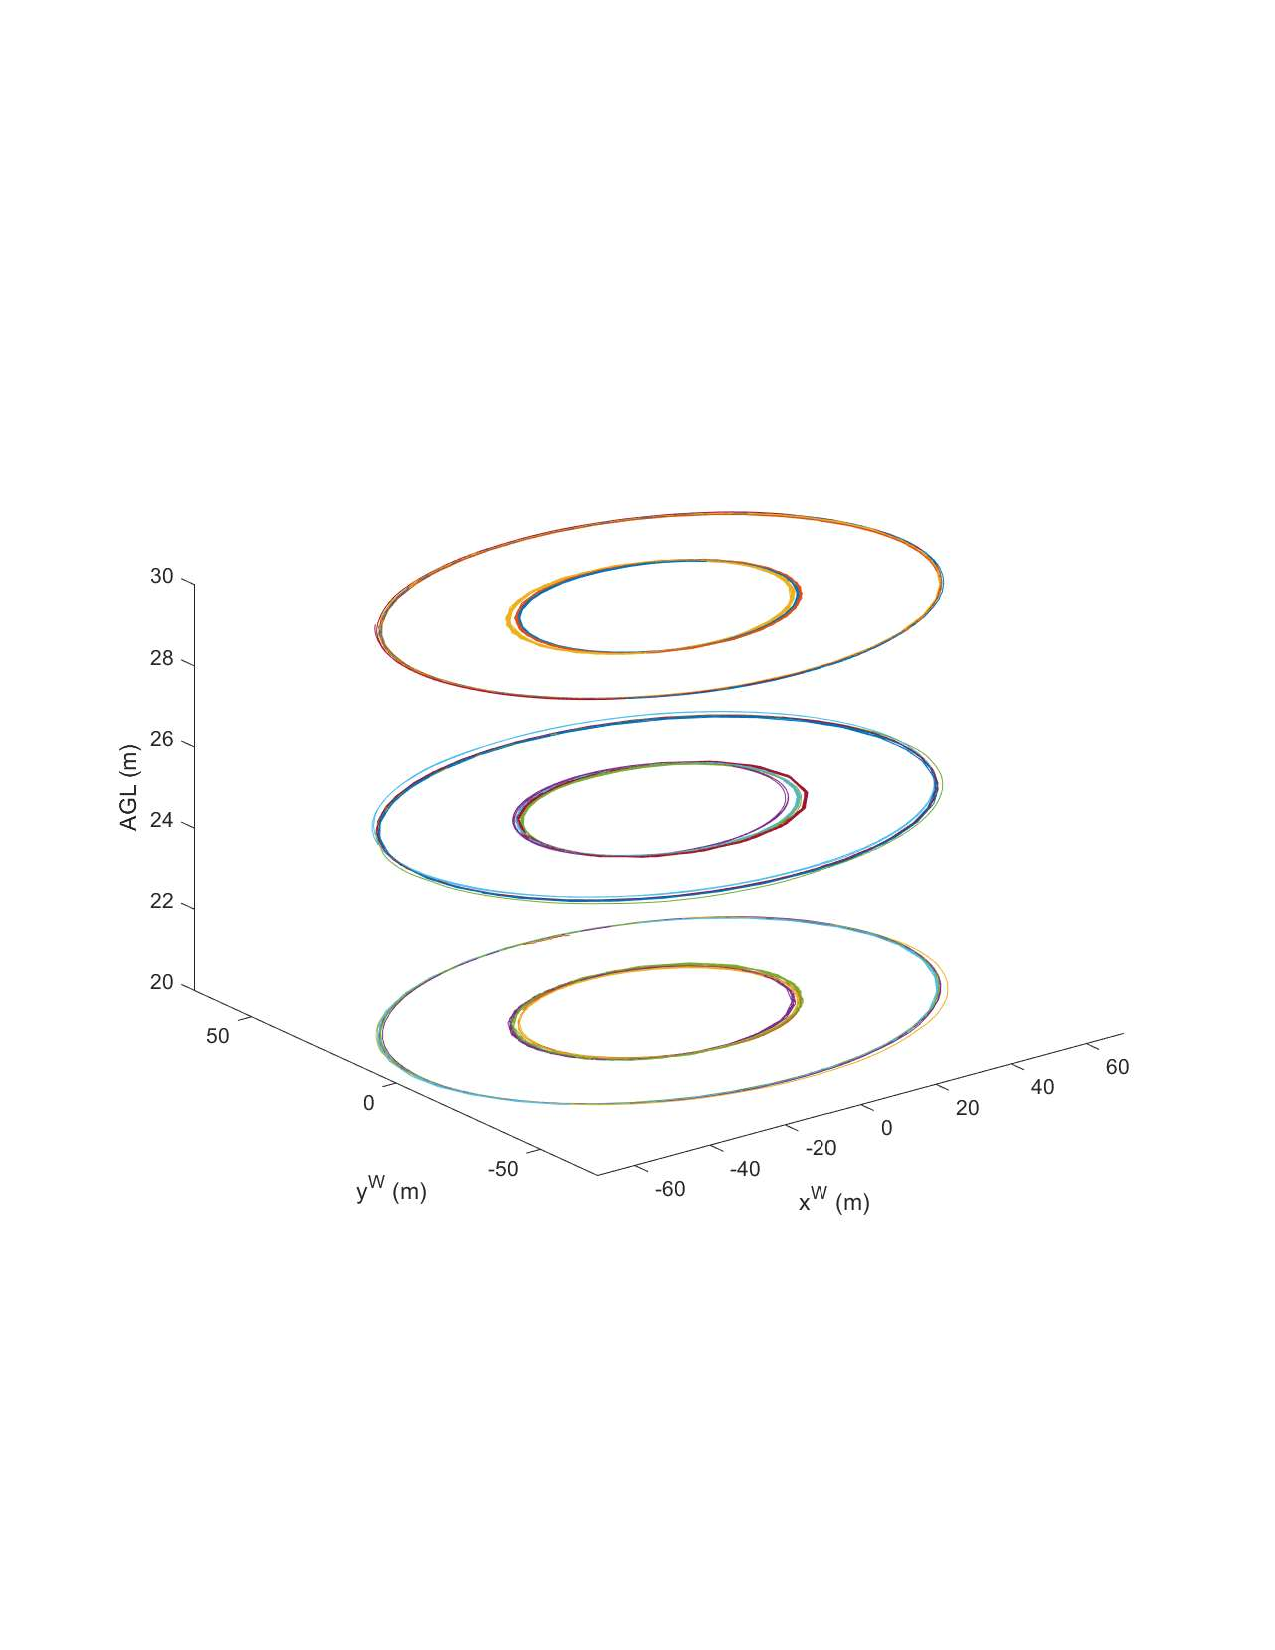
\includegraphics[width=0.5\textwidth, trim={2cm 7.5cm 1cm 8cm},clip]{expSchematic.pdf}
	\caption{Position data from all our flight experiments. With 2 orbit radii, 3 altitudes, and 5 linear ground velocities we collected data for 30 different trajectories. Each trajectory was flown for approximately 120 seconds giving us 97 complete orbits to analyze. All flight data and our ROS package can be found at https://github.com/alex-faustino/brg-qr-OptEnd.}
\end{figure}

Currently, most approaches to solving this problem can be classified into the development of either hardware, algorithm (software) \cite{di2015energy,ware2016analysis,tagliabue2019model}, or bio-inspired/hybrid systems. Traditionally, the bulk of work done to increase quadrotor efficiency is in the first category. Efforts here consist mostly of reducing the weight of materials such as the airframe, sensors, and power electronics. The second category contains methods that incorporate vehicle power consumption into cost functions of existing optimal planning and control algorithms. Finally, the third category often produces novel systems that increase efficiency by transitioning to another dynamic mode such as perching, walking, or rolling. In \cite{karydis2017energetics}, Karydis et al. provide a thorough review of promising work in all three categories. 

This paper contributes to the second category, the popularity of which has grown in recent years due to the increased capabilities of onboard computers. Since the majority of algorithmic approaches are model-based, their performance is directly related to how well their power consumption model can estimate the true power consumed in actual flight. Several white box \cite{liu2017power, bezzo2016online} and black box \cite{di2015energy, prasetia2019mission} models have been proposed in recent years each with their own drawbacks. 

The benefit of black box models is that they remove the need for a theoretical model, which would require determining numerous physical parameters about the quadrotor. However, they do not generalize to any desired trajectory; this constrains motion planning methods to the set of predetermined models. While these models have shown promise in implementation, this paper focuses on the study of white box models. 

White box models primarily consist of summing some combination of the four major sources of aerodynamic power -- induced, parasitic, profile, and climb -- which are each covered in more detail in \ref{sec:Power}. Depending on which terms a model includes and how it approximates them, the model either sacrifices accuracy or requires several parameters to be identified about the quadrotor beforehand. 

Our paper makes three contributions:
\begin{enumerate}
	\item It provides a parametric model of quadrotor power consumption that performs better than existing models.
	\item It shows the impact of each power term on the accuracy of the model using an ablation study with data from outdoor flight tests.
	\item It releases the data from these flight tests for others to use freely as a benchmark.
\end{enumerate} 
Section \ref{sec:Related} talks in more detail about existing methods that use black box or white box power consumption models; Section \ref{sec:Dynamics} presents our dynamic model, in particular our model of aerodynamic drag; Section \ref{sec:Power} presents our power consumption model; Section \ref{sec:Exp} describes our flight experiments; Section \ref{sec:Results} describes the results of our experiments and discusses their significance; Section \ref{sec:Future} concludes with a consideration of practical applications.






